% Generated from ../chapters/11-endogenous-escape-velocity.md
\chapter{Endogenous Escape Velocity}\label{chapter-11-endogenous-escape-velocity}

Longevity escape velocity is usually technological. Better therapies buy time for the next generation of therapies. The organism remains dependent on repeated external repair.

The parallel proposed here is \textbf{endogenous maintenance escape velocity}: a regime in which the organism's effective repair, clearance, and adaptation improve enough to exceed the rate at which damage and loss of reserve accumulate.

The idea must be formulated carefully. If repair exceeds damage by a fixed amount, damage falls linearly until it reaches a floor. Runaway improvement requires feedback: better health must increase the capacity to become healthier.

Let $H(t)$ represent adaptive reserve and $D(t)$ represent effective damage burden. A minimal conceptual model is

\[\frac{dH}{dt}=A(H,L,R)-B(D,H),\]

\[\frac{dD}{dt}=G(H,t)-Q(H,R,D).\]

Here $L$ is adaptive load and $R$ is recovery resource. $A$ represents gains from appropriately dosed challenge and recovery. $B$ represents losses imposed by damage and overload. $G$ is new damage generation, and $Q$ is repair or clearance.

The equations are not fitted biological laws. They force us to state the hypothesis. Positive feedback exists if a rise in $H$ increases future $A$ or $Q$, or decreases $G$. Negative feedback and saturation also matter. Excessive loading can reduce reserve. Repair mechanisms have finite capacity. Some damage may be inaccessible.

A plausible trajectory is therefore logistic rather than unbounded. Improvement may begin slowly while constraints remain, accelerate after a transition, and plateau near tissue-specific limits.

\begin{figure}
\centering
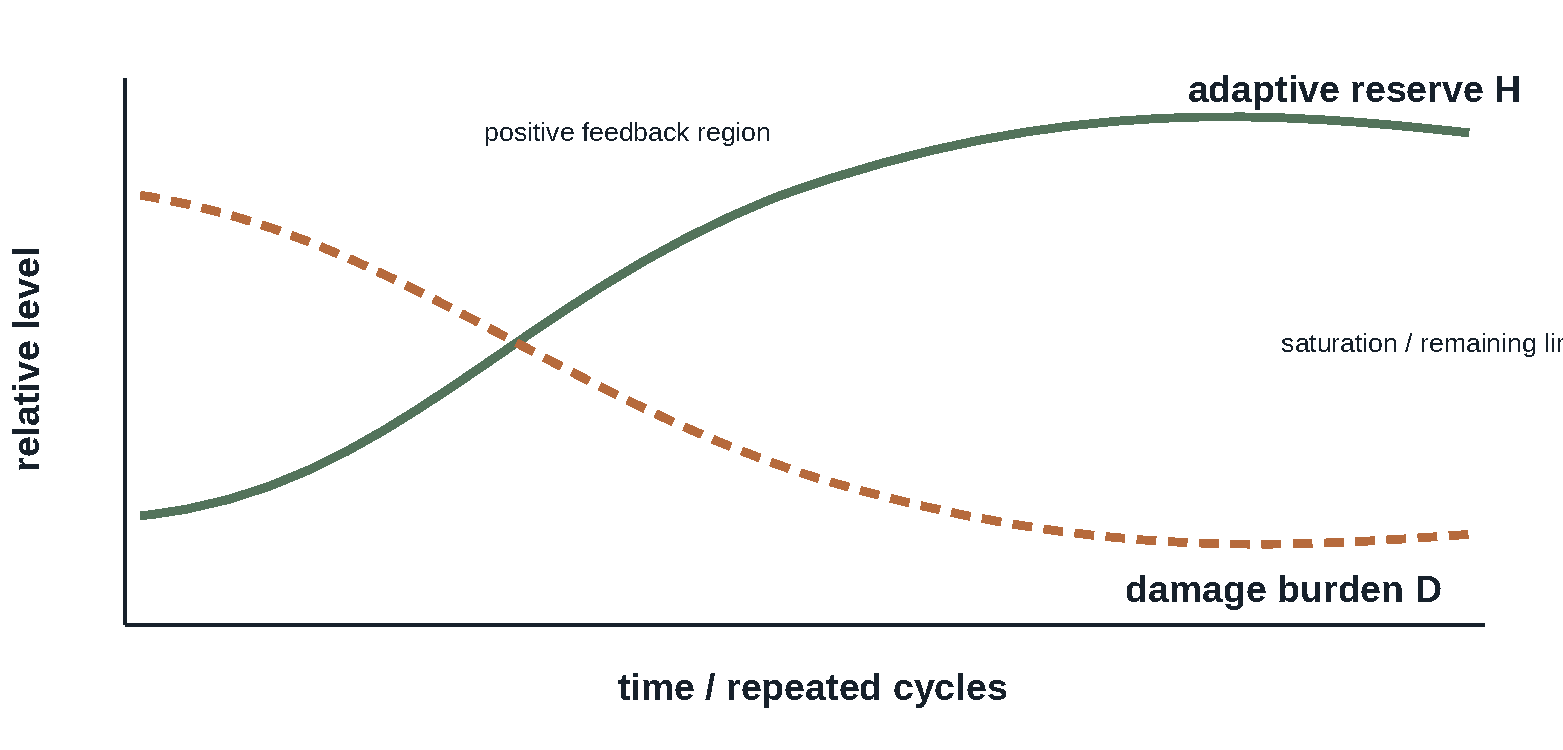
\includegraphics[width=0.9\textwidth,height=.68\textheight]{../figures/reserve-damage-model.pdf}
\caption{A conceptual model of reserve and damage. Positive feedback can improve future repair, but overload, saturation, and irreducible damage create limits.}\label{fig:reserve}
\end{figure}

The testable prediction is second-order. A successful cycle should not only improve a state variable. It should improve the response to the next comparable challenge. If strength training, relaxation, sleep, and metabolic cycling increase adaptive reserve, later training and recovery should become more effective.

The strong claim---indefinite endogenous rejuvenation---has no human evidence. The weaker claim is already useful: interventions should be evaluated by whether they preserve or enlarge adaptive capacity, not merely by whether they temporarily improve a biomarker.
